\documentclass[12pt]{article}
%\usepackage{alltt}
\usepackage[utf8]{inputenc}
\usepackage[dvips]{graphicx}
%\usepackage{a4wide}
\usepackage{epsfig}
\usepackage{fancybox}
\usepackage{verbatim}
\usepackage{array}
\usepackage{latexsym}
\usepackage{alltt}
%\usepackage{dsfont}
\usepackage{caption}
\usepackage{subcaption}
%\usepackage{fullpage}
\usepackage{hyperref}
\usepackage{textcomp}
\usepackage{listings}
\usepackage{color}
\usepackage{amsmath}
\usepackage{amsfonts}
\usepackage{tikz}
\usepackage{float}
\usepackage[hmargin=3cm,vmargin=5.0cm]{geometry}
%\topmargin=0cm
\topmargin=-1.8cm
\addtolength{\textheight}{6.5cm}
\addtolength{\textwidth}{2.0cm}
%\setlength{\leftmargin}{-5cm}
\setlength{\oddsidemargin}{0.0cm}
\setlength{\evensidemargin}{0.0cm}

\newcommand{\HRule}{\rule{\linewidth}{1mm}}
\newcommand{\kutu}[2]{\framebox[#1mm]{\rule[-2mm]{0mm}{#2mm}}}
\newcommand{\gap}{ \\[1mm] }

\newcommand{\Q}{\raisebox{1.7pt}{$\scriptstyle\bigcirc$}}

\lstset{
    %backgroundcolor=\color{lbcolor},
    tabsize=2,
    language=C++,
    basicstyle=\footnotesize,
    numberstyle=\footnotesize,
    aboveskip={0.0\baselineskip},
    belowskip={0.0\baselineskip},
    columns=fixed,
    showstringspaces=false,
    breaklines=true,
    prebreak=\raisebox{0ex}[0ex][0ex]{\ensuremath{\hookleftarrow}},
    %frame=single,
    showtabs=false,
    showspaces=false,
    showstringspaces=false,
    identifierstyle=\ttfamily,
    keywordstyle=\color[rgb]{0,0,1},
    commentstyle=\color[rgb]{0.133,0.545,0.133},
    stringstyle=\color[rgb]{0.627,0.126,0.941},
}


\begin{document}



\noindent
\begin{center}
                    \Large Take Home Exam 5 Figures
\end{center}







\section*{Question 1 Figures}
\begin{figure}[H]
	\centering
	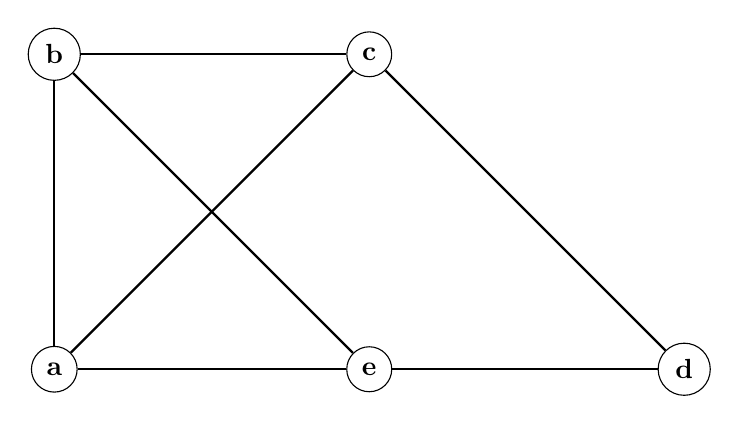
\begin{tikzpicture}
	
	\node[shape=circle,draw=black] (b) at (0, 4)     {\textbf{b}};
	\node[shape=circle,draw=black] (c) at (4, 4)     {\textbf{c}};
	\node[shape=circle,draw=black] (d) at (8, 0)     {\textbf{d}};
	\node[shape=circle,draw=black] (e) at (4, 0)     {\textbf{e}};
	\node[shape=circle,draw=black] (a) at (0, 0)     {\textbf{a}};
	
	\path[-, thick] (a) edge (e);
	\path[-, thick] (e) edge (d);
	\path[-, thick] (c) edge (d);
	\path[-, thick] (b) edge (c);
	\path[-, thick] (a) edge (b);
	\path[-, thick] (a) edge (c);
	\path[-, thick] (b) edge (e);
	
	\end{tikzpicture} 
	\caption{Graph G in Q1.}	
	\label{fig:g1}
\end{figure}


\section*{Question 2 Figures}

\begin{figure}[H]
	\centering
	\begin{subfigure}[b]{0.4\textwidth}
         \centering
         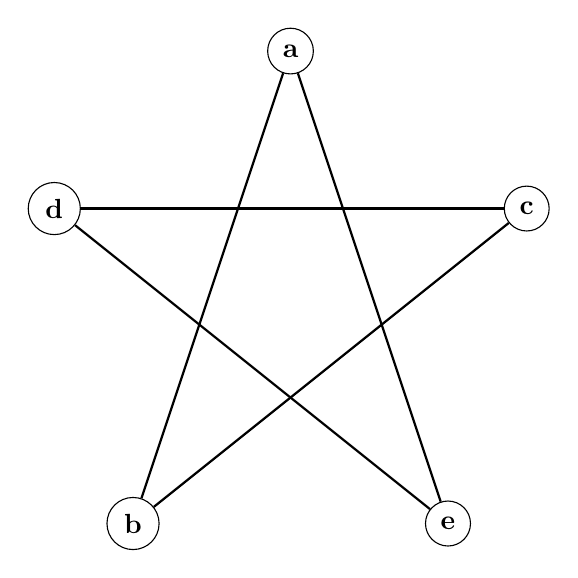
\begin{tikzpicture}
	
	\node[shape=circle,draw=black] (b) at (2, 0)     {\textbf{b}};
	\node[shape=circle,draw=black] (e) at (6, 0)     {\textbf{e}};
	\node[shape=circle,draw=black] (d) at (1, 4)     {\textbf{d}};
	\node[shape=circle,draw=black] (c) at (7, 4)     {\textbf{c}};
	\node[shape=circle,draw=black] (a) at (4, 6)     {\textbf{a}};
	
	\path[-, thick] (a) edge (b);
	\path[-, thick] (b) edge (c);
	\path[-, thick] (c) edge (d);
	\path[-, thick] (d) edge (e);
	\path[-, thick] (e) edge (a);
	
	\end{tikzpicture} 
         \caption{G}
         \label{fig:g}
     \end{subfigure}
     \hfill
     \begin{subfigure}[b]{0.4\textwidth}
         \centering
         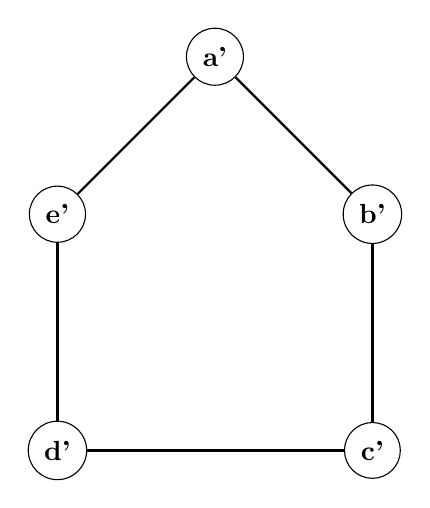
\begin{tikzpicture}
	
	\node[shape=circle,draw=black] (d') at (2, 0)     {\textbf{d'}};
	\node[shape=circle,draw=black] (c') at (6, 0)     {\textbf{c'}};
	\node[shape=circle,draw=black] (e') at (2, 3)     {\textbf{e'}};
	\node[shape=circle,draw=black] (b') at (6, 3)     {\textbf{b'}};
	\node[shape=circle,draw=black] (a') at (4, 5)     {\textbf{a'}};
	
    \path[-, thick] (a') edge (b');
    \path[-, thick] (a') edge (e');
    \path[-, thick] (b') edge (c');
    \path[-, thick] (d') edge (e');
    \path[-, thick] (c') edge (d');
	
	\end{tikzpicture} 
         \caption{H}
         \label{fig:h}
     \end{subfigure}
     \caption{Graph G and H in Q2.}
        \label{fig:g2}
\end{figure}


\section*{Question 3 Figures}

\begin{figure}[H]
	\centering
	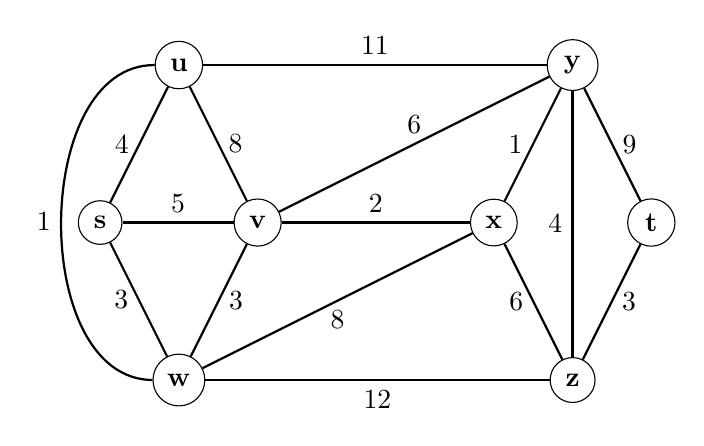
\begin{tikzpicture}
	
	\node[shape=circle,draw=black] (s) at (-1, 2)     {\textbf{s}};
	\node[shape=circle,draw=black] (u) at (0, 4)     {\textbf{u}};
	\node[shape=circle,draw=black] (y) at (5, 4)     {\textbf{y}};
	\node[shape=circle,draw=black] (w) at (0, 0)     {\textbf{w}};
	\node[shape=circle,draw=black] (z) at (5, 0)     {\textbf{z}};
	\node[shape=circle,draw=black] (v) at (1, 2)     {\textbf{v}};
    \node[shape=circle,draw=black] (x) at (4, 2)     {\textbf{x}};
    \node[shape=circle,draw=black] (t) at (6, 2)     {\textbf{t}};
 
	\path[-, thick] (u) edge [bend right=90] node[left]{1} (w);
	\path[-, thick] (s) edge node[left]{4} (u);
	\path[-, thick] (s) edge node[above]{5} (v);
	\path[-, thick] (u) edge node[right]{8} (v);
	\path[-, thick] (s) edge node[left]{3} (w);
	\path[-, thick] (v) edge node[right]{3} (w);
	\path[-, thick] (u) edge node[above]{11} (y);
	\path[-, thick] (y) edge node[right]{9} (t);
	\path[-, thick] (y) edge node[left]{1} (x);
	\path[-, thick] (y) edge node[left]{4} (z);
	\path[-, thick] (x) edge node[left]{6} (z);
	\path[-, thick] (t) edge node[right]{3} (z);
	\path[-, thick] (w) edge node[below]{12} (z);
	\path[-, thick] (x) edge node[below]{8} (w);
	\path[-, thick] (v) edge node[above]{2} (x);
	\path[-, thick] (v) edge node[above]{6} (y);
	
	\end{tikzpicture} 
	\caption{Graph G in Q3.}	
	\label{fig:g3}
\end{figure}

\section*{Question 4 Figures}

\begin{figure}[H]
	\centering
	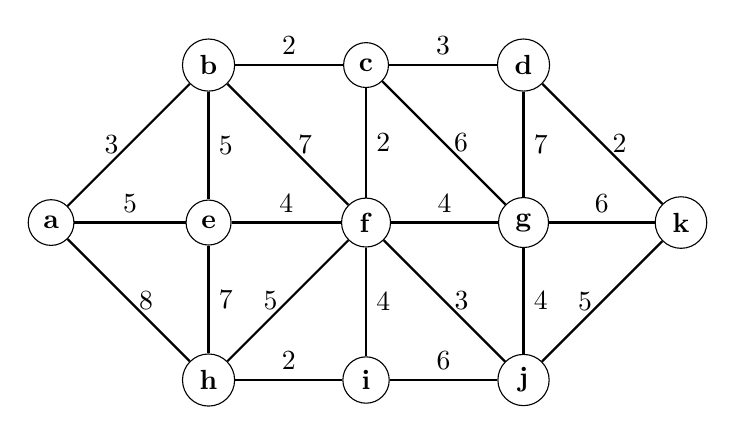
\begin{tikzpicture}
	
	\node[shape=circle,draw=black] (a) at (-2, 2)     {\textbf{a}};
	\node[shape=circle,draw=black] (b) at (0, 4)     {\textbf{b}};
	\node[shape=circle,draw=black] (c) at (2, 4)     {\textbf{c}};
	\node[shape=circle,draw=black] (d) at (4, 4)     {\textbf{d}};
	\node[shape=circle,draw=black] (e) at (0, 2)     {\textbf{e}};
	\node[shape=circle,draw=black] (f) at (2, 2)     {\textbf{f}};
	\node[shape=circle,draw=black] (g) at (4, 2)     {\textbf{g}};
	\node[shape=circle,draw=black] (h) at (0, 0)     {\textbf{h}};
	\node[shape=circle,draw=black] (i) at (2, 0)     {\textbf{i}};
	\node[shape=circle,draw=black] (j) at (4, 0)     {\textbf{j}};
	\node[shape=circle,draw=black] (k) at (6, 2)     {\textbf{k}};
	
	\path[-, thick] (a) edge node[left]{3} (b);
	\path[-, thick] (a) edge node[above]{5} (e);
	\path[-, thick] (a) edge node[right]{8} (h);
	\path[-, thick] (b) edge node[above]{2} (c);
	\path[-, thick] (b) edge node[right]{5} (e);
	\path[-, thick] (b) edge node[right]{7} (f);
	\path[-, thick] (c) edge node[above]{3} (d);
	\path[-, thick] (c) edge node[right]{2} (f);
	\path[-, thick] (c) edge node[right]{6} (g);
	\path[-, thick] (d) edge node[right]{7} (g);
	\path[-, thick] (d) edge node[right]{2} (k);
	\path[-, thick] (e) edge node[above]{4} (f);
	\path[-, thick] (e) edge node[right]{7} (h);
	\path[-, thick] (f) edge node[above]{4} (g);
	\path[-, thick] (f) edge node[left]{5} (h);
	\path[-, thick] (f) edge node[right]{4} (i);
	\path[-, thick] (f) edge node[right]{3} (j);
	\path[-, thick] (g) edge node[right]{4} (j);
	\path[-, thick] (g) edge node[above]{6} (k);
	\path[-, thick] (h) edge node[above]{2} (i);
	\path[-, thick] (i) edge node[above]{6} (j);
	\path[-, thick] (j) edge node[left]{5} (k);
	
	\end{tikzpicture} 
	\caption{Graph G in Q4.}	
	\label{fig:g4}
\end{figure}



\end{document}

